\documentclass[a4paper]{book}

% Packages
\usepackage{graphicx}
\usepackage{geometry}
\usepackage{hyperref}
\usepackage[utf8]{vietnam}
\usepackage{amsmath}

% Geometry setup
\geometry{left=2cm,right=2cm,top=2cm,bottom=2cm}

% Titlepage information
\newcommand{\reporttitle}{Employee-Attendance-System-Using-Camera}
\newcommand{\reportauthors}{%
    Nguyễn Hữu Duy
}
\newcommand{\courseinfo}{Mã học phần: MAT3508\\ Học kỳ 1, Năm học 2025-2026}
\newcommand{\universitylogo}{HUS.png} % Đặt file logo vào cùng thư mục

\newcommand{\doi}[1]{\href{https://doi.org/#1}{\texttt{#1}}} % DOI link command


% Loại bỏ trang trắng thừa đầu chương (book class)
\let\cleardoublepage\clearpage
\begin{document}

% Trang bìa
\begin{titlepage}
    \centering
    \vspace*{-1cm}
    {\LARGE\MakeUppercase{Đại học Quốc gia Hà Nội}\par}
    {\LARGE\MakeUppercase{Trường Đại học Khoa học Tự nhiên}\par}
    \vfill
    \includegraphics[width=0.3\textwidth]{\universitylogo}\par\vfill
    {\Huge \bfseries \reporttitle \par}
    \vspace{1cm}
    {\Large \reportauthors \par}
    \vspace{1cm}
    {\large \courseinfo \par}
    \vfill
\end{titlepage}

% Trang thông tin dự án
\clearpage
\thispagestyle{empty}
\begin{center}
    {\LARGE \textbf{Thông tin Dự án}}\\[1.5em]
    \parbox{0.85\textwidth}{
        \textit{[Thông tin này cũng cần được ghi trong README.md của kho GitHub.]}
    }
    \\[2em]
    \begin{tabular}{rl}
        \textbf{Học phần:} & MAT3508 -- Nhập môn Trí tuệ Nhân tạo \\
        \textbf{Học kỳ:} & Học kỳ 1, Năm học 2025-2026 \\
        \textbf{Trường:} & VNU-HUS (Đại học Quốc gia Hà Nội -- Trường Đại học Khoa học Tự nhiên) \\
        \textbf{Tên dự án:} & {[Nhận diện khuôn mặt]} \\
        \textbf{Ngày nộp:} & 30/11/2025 \\
        \textbf{Báo cáo PDF:} & \href{[PDF Link]}{Liên kết tới báo cáo PDF trong kho GitHub} \\
        \textbf{Slide thuyết trình:} & \href{[Slides Link]}{Liên kết tới slide thuyết trình trong kho GitHub} \\
        \textbf{Kho GitHub:} & \url{[GitHub Repository URL]}
    \end{tabular}
    \\[2em]
    {\Large \textbf{Thành viên nhóm}}\\[1em]
    \begin{tabular}{|l|l|l|l|}
        \hline
        \textbf{Họ tên} & \textbf{Mã sinh viên} & \textbf{Tên GitHub}  \\
        \hline
        (Nguyễn Hữu Duy) & (23001853) & (23001853-wq)  \\
        \hline
     
    \end{tabular}
\end{center}

% Gom mục lục, danh sách hình, danh sách bảng vào một chỗ, chỉ clearpage sau cùng để tránh sinh trang trắng thừa
	ableofcontents
\listoffigures
\listoftables
\clearpage

% Chương 1: Giới thiệu
\chapter{Giới thiệu}

\section{Tóm tắt}
Hệ thống điểm danh tự động dựa trên nhận diện khuôn mặt sử dụng học sâu (Deep Learning) được phát triển nhằm thay thế phương pháp điểm danh thủ công, nâng cao độ chính xác và tự động hóa. Dữ liệu khuôn mặt được thu thập qua webcam, tiền xử lý và lưu trữ, trước khi trích xuất đặc trưng bằng mạng MobileNetV2. Các vector đặc trưng 1280 chiều sau đó được **chuẩn hóa L2** để đảm bảo độ ổn định và độ chính xác khi đưa vào các thuật toán phân loại.

Trước khi trích xuất vector, hệ thống sử dụng thuật toán Haar Cascade của OpenCV để phát hiện và cắt vùng khuôn mặt, giúp xử lý tốt các điều kiện ánh sáng khác nhau và đảm bảo vector đầu vào chỉ chứa khuôn mặt. Các thuật toán phân loại được áp dụng gồm: SVM, KNN, Random Forest (học có giám sát) và Cosine Similarity, L2 Distance (học không giám sát), từ đó so sánh để lựa chọn giải pháp tối ưu.

Kết quả thực nghiệm cho thấy SVM (RBF Kernel) kết hợp chuẩn hóa L2 đạt độ chính xác cao nhất, nhận diện ổn định, thời gian xử lý nhanh và phù hợp triển khai thực tế. Hệ thống còn có giao diện \textbf{Streamlit} thân thiện, tích hợp cơ sở dữ liệu \textbf{SQL Server} để quản lý thông tin nhân viên và lịch sử điểm danh, đồng thời hỗ trợ tăng cường dữ liệu tự động nhằm cải thiện hiệu quả nhận diện.

\section{Bài toán đặt ra}
Điểm danh truyền thống bằng giấy tờ hoặc thẻ từ dễ gian lận, tốn thời gian và không phù hợp với quá trình chuyển đổi số. Bài toán đặt ra là xây dựng hệ thống điểm danh tự động, nhận diện chính xác khuôn mặt nhân viên trong điều kiện thực tế, đảm bảo an ninh, dễ sử dụng và có khả năng mở rộng.

\section{Thách thức}
Hệ thống cần giải quyết các thách thức sau:
\begin{enumerate}
    \item \textbf{Đảm bảo độ chính xác cao với dữ liệu nhỏ:} Số lượng ảnh mỗi nhân viên ít, cần thuật toán học sâu nhẹ kết hợp SVM/KNN/RF để đạt hiệu quả mà không quá khớp.
    \item \textbf{Xử lý đa dạng khuôn mặt và điều kiện ánh sáng:} Haar Cascade giúp phát hiện và cắt khuôn mặt, chuẩn hóa ảnh trước khi trích xuất vector.
    \item \textbf{Chuẩn hóa L2 và tối ưu tốc độ nhận diện:} Vector 1280 chiều từ MobileNetV2 được chuẩn hóa L2 và đưa vào SVM cho phép nhận diện nhanh, đủ cho ứng dụng real-time.
    \item \textbf{So sánh nhiều thuật toán:} Học có giám sát và không giám sát để chọn mô hình tối ưu về độ chính xác, tốc độ và khả năng mở rộng.
    \item \textbf{Quản lý check-in/check-out và cơ sở dữ liệu:} Sau khi nhận diện, hệ thống ghi nhận thời gian vào/ra nhân viên vào SQL Server, hỗ trợ tra cứu lịch sử và báo cáo.
    \item \textbf{Khả năng mở rộng:} Thiết kế để mở rộng khi số lượng nhân viên tăng hoặc dữ liệu lớn hơn, dễ tích hợp các thuật toán Deep Learning nâng cao như ArcFace.
\end{enumerate}


% Chương 2: Phương pháp & Triển khai
\chapter{Phương pháp \& Triển khai}

\section{Phương pháp}
Pipeline nhận diện khuôn mặt gồm các bước chính sau:

\begin{enumerate}
    \item \textbf{Thu thập dữ liệu:} Sử dụng webcam để chụp ảnh khuôn mặt nhân viên. Mỗi nhân viên có khoảng 50 ảnh, ghi chú thông tin ID.
    
    \item \textbf{Phát hiện và cắt khuôn mặt:} Áp dụng thuật toán Haar Cascade (OpenCV) để xác định vị trí khuôn mặt trong ảnh, loại bỏ nền và các đối tượng không liên quan.\\
    \textbf{Công thức đặc trưng Haar (tóm tắt):}
    \[
    H = \sum_{\text{pixel vùng sáng}} I - \sum_{\text{pixel vùng tối}} I
    \]
    
    \item \textbf{Tiền xử lý và tăng cường dữ liệu:} 
    \begin{itemize}
        \item Chuẩn hóa kích thước ảnh về 224x224 px.
        \item Tăng cường dữ liệu bằng các phép xoay, lật, thay đổi sáng/tối.
    \end{itemize}
    
    \item \textbf{Trích xuất đặc trưng:} 
    \begin{itemize}
        \item Sử dụng MobileNetV2 pretrained để trích xuất vector đặc trưng 1280 chiều.
        \item Thực hiện \textbf{chuẩn hóa L2}:
        \[
        v_{\text{norm}} = \frac{v}{\|v\|_2} = \frac{v}{\sqrt{\sum_{i=1}^{1280} v_i^2}}
        \]
        \item Gán nhãn dữ liệu dựa trên ID nhân viên.
    \end{itemize}

    \item \textbf{Phân loại:} So sánh 5 thuật toán với công thức chính:
    \begin{itemize}
        \item \textbf{SVM (RBF Kernel):} 
        \[
        f(x) = \text{sign}(w^T x + b), \quad 
        K(x_i, x_j) = \exp(-\gamma \|x_i - x_j\|^2)
        \]
        \item \textbf{KNN:} 
        \[
        \text{label}(x) = \text{mode}(\{ \text{label}(x_i) \mid x_i \in k\text{ nearest neighbors} \})
        \]
        \item \textbf{Random Forest:} Dự đoán theo đa số phiếu từ nhiều cây quyết định.
        \item \textbf{Cosine Similarity:} 
        \[
        \cos(\theta) = \frac{a \cdot b}{\|a\|_2 \|b\|_2}
        \]
        \item \textbf{L2 Distance:} 
        \[
        d(a, b) = \sqrt{\sum_{i=1}^{1280} (a_i - b_i)^2}
        \]
    \end{itemize}
    
    \item \textbf{Đánh giá và chọn mô hình tối ưu:} Sử dụng tập test để đo độ chính xác và thời gian, xác định SVM (RBF Kernel) là mô hình tối ưu.
\end{enumerate}

\section{Triển khai}
Hệ thống triển khai với các thành phần chính:

\begin{itemize}
    \item \textbf{Thu thập và lưu trữ dữ liệu:} Script Python kết hợp OpenCV và Haar Cascade, lưu ảnh khuôn mặt từng nhân viên.
    
    \item \textbf{Tiền xử lý và tăng cường:} Sử dụng \texttt{ImageDataGenerator} của Keras để sinh thêm dữ liệu và chuẩn hóa ảnh.
    
    \item \textbf{Trích xuất đặc trưng:} MobileNetV2 pretrained, vector 1280 chiều, chuẩn hóa L2.
    
    \item \textbf{Huấn luyện mô hình:} Sử dụng scikit-learn cho SVM, KNN, Random Forest. So sánh với Cosine và L2 template matching.
    
    \item \textbf{Nhận diện thực tế:} Ứng dụng Streamlit làm giao diện web, nhận diện real-time từ webcam, hiển thị tên và ID nhân viên, đồng thời ghi check-in/check-out vào cơ sở dữ liệu SQL Server.
    
    \item \textbf{Lưu trữ kết quả:} Model và label map lưu dưới dạng file \texttt{.pkl}; thông tin nhân viên và lịch sử điểm danh lưu SQL Server.
    
    \item \textbf{Thư viện và công nghệ:} TensorFlow/Keras, scikit-learn, OpenCV, pandas, streamlit, pyodbc.
\end{itemize}

% Chương 3: Kết quả & Phân tích
\chapter{Kết quả \& Phân tích}

\section{Minh họa dữ liệu}
Một số ảnh đại diện trong tập huấn luyện được trình bày dưới đây để minh họa đa dạng khuôn mặt và điều kiện ánh sáng:

\begin{figure}[h!]
    \centering
    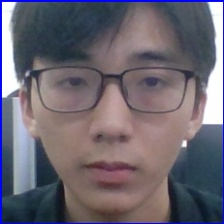
\includegraphics[width=0.2\textwidth]{User.1.1.jpg}
    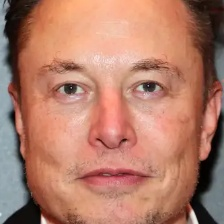
\includegraphics[width=0.2\textwidth]{User.2.2.jpg}
    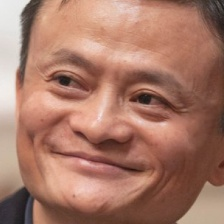
\includegraphics[width=0.2\textwidth]{User.4.1.jpg}
    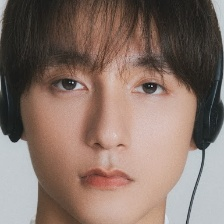
\includegraphics[width=0.2\textwidth]{User.5.3.jpg}
    \caption{Ảnh minh họa một số nhân viên trong tập huấn luyện}
    \label{fig:sample_images}
\end{figure}

\section{So sánh thuật toán}
Bảng dưới đây tổng hợp kết quả thực nghiệm trên tập test (7 nhân viên, mỗi người 10 ảnh) với 5 thuật toán:

\begin{figure}[h!]
    \centering
    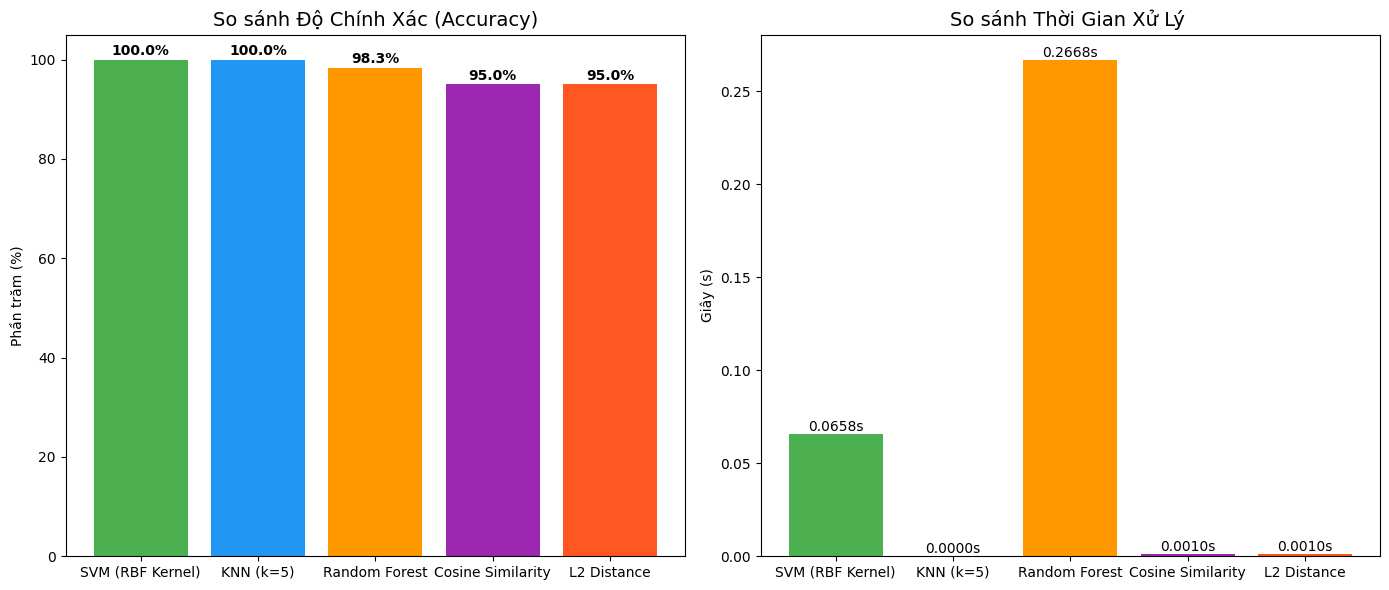
\includegraphics[width=0.9\textwidth]{model.png}
    \caption{So sánh độ chính xác và thời gian thực thi của các thuật toán}
    \label{fig:model-compare}
\end{figure}

\begin{table}[h!]
\centering
\begin{tabular}{lccc}
\hline
	extbf{Thuật toán} & \textbf{Độ chính xác (\%)} & \textbf{Thời gian xử lý (s)} & \textbf{Ghi chú} \\
\hline
SVM (RBF Kernel)     & 100      & 0.07   & Tốt nhất, ổn định \\
KNN (k=5)            & 100      & 0.001  & Dữ liệu ít hiệu quả, kém ổn định khi dữ liệu tăng \\
Random Forest        & 98.3     & 0.27   & Kháng nhiễu tốt, nhưng độ chính xác thấp hơn SVM \\
Cosine Similarity    & 98.3     & 0.001  & Học không giám sát, dễ áp dụng với dữ liệu ít \\
L2 Distance          & 98.3     & 0.001  & Học không giám sát, hiệu quả gần giống Cosine \\
\hline
\end{tabular}
\caption{Bảng so sánh các thuật toán nhận diện khuôn mặt}
\label{tab:model-compare}
\end{table}

\section{Phân tích kết quả}
\begin{itemize}
    \item \textbf{SVM (RBF Kernel):} Đạt 100\% độ chính xác nhờ khả năng phân tách tốt, tổng quát hóa mạnh và kết hợp chuẩn hóa L2. Thời gian xử lý chấp nhận được cho real-time.
    
    \item \textbf{KNN:} Với k=3 hoặc k=5, độ chính xác đạt 100\% trên tập test nhỏ, nhưng khi k tăng hoặc dữ liệu nhiều, hiệu quả giảm. Dễ bị nhạy cảm với nhiễu.
    
    \item \textbf{Random Forest:} Kháng nhiễu tốt nhưng chưa tối ưu với vector đặc trưng 1280 chiều, dẫn đến độ chính xác thấp hơn SVM.
    
    \item \textbf{Cosine Similarity \& L2 Distance:} Học không giám sát, phù hợp khi số ảnh mỗi nhân viên ít. Hiệu quả gần bằng học có giám sát nhưng tốc độ và độ chính xác kém ổn định hơn với dữ liệu lớn hoặc phức tạp.
    
    \item \textbf{Thời gian xử lý:} Cosine và L2 nhanh hơn nhiều nhưng SVM vẫn đủ nhanh cho ứng dụng real-time. KNN quá nhanh nhưng không ổn định khi dữ liệu tăng. Random Forest chậm nhất trong các thuật toán.
\end{itemize}
\section{Kết quả nhận diện thực tế với SVM}

Để đánh giá khả năng hoạt động của hệ thống trong bối cảnh thực tế, các ảnh trong \textbf{File 03} (tập kiểm thử độc lập, không tham gia huấn luyện) được đưa vào mô hình phân loại \textbf{SVM (RBF Kernel)}. 

Trong giai đoạn nhận diện, hệ thống thực hiện quy trình sau:

\begin{enumerate}
    \item \textbf{Phát hiện khuôn mặt} bằng Haar Cascade và cắt vùng ROI.
    \item \textbf{Trích xuất đặc trưng}:  
    Sử dụng MobileNetV2 (pretrained ImageNet) để lấy vector 1280 chiều và chuẩn hoá L2.
    \item \textbf{Dự đoán bằng SVM}:  
    \begin{itemize}
        \item Lấy \textbf{ID dự đoán} từ mô hình.
        \item Lấy \textbf{độ tin cậy} bằng hàm \texttt{predict\_proba}.
    \end{itemize}
    \item \textbf{Áp dụng ngưỡng tin cậy 0.55}:  
    Nếu xác suất < 0.55 → gán nhãn \textit{Unknown}.
    \item \textbf{Truy vấn thông tin nhân viên từ SQL Server} dựa theo ID trả về tên khi nhận diện.
% (Không có danh sách con ở đây, xóa itemize rỗng)
\end{enumerate}

Kết quả nhận diện được thể hiện dưới đây:

\begin{figure}[h!]
    \centering
    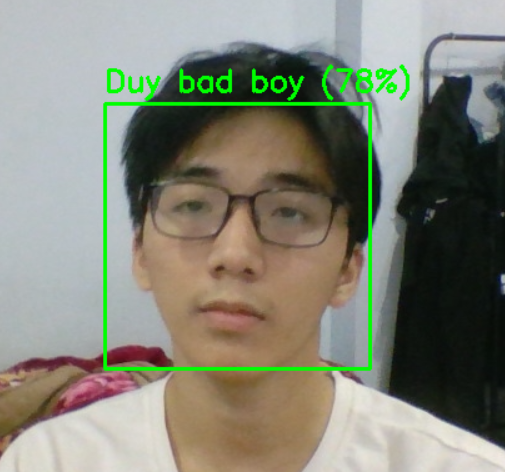
\includegraphics[width=0.2\textwidth]{nv1.png}
    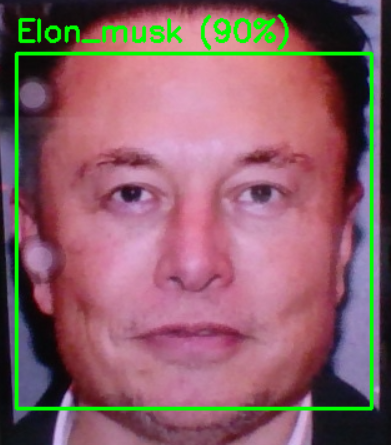
\includegraphics[width=0.2\textwidth]{nv2.png}
    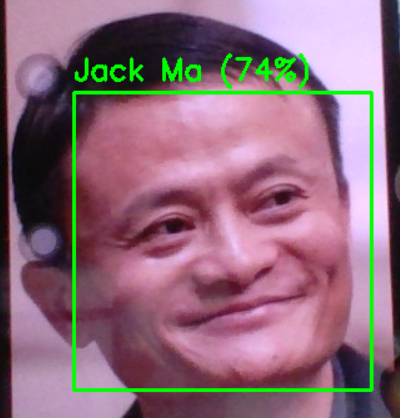
\includegraphics[width=0.2\textwidth]{nv4.png}
    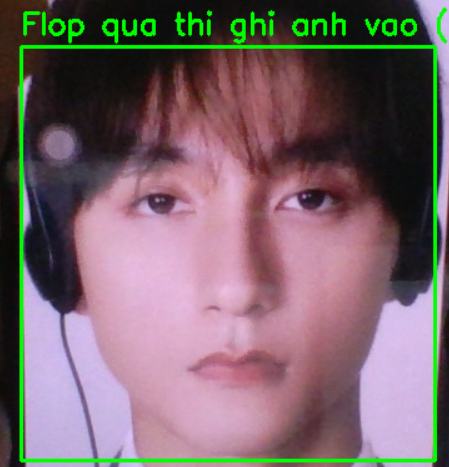
\includegraphics[width=0.2\textwidth]{nv5.png}
    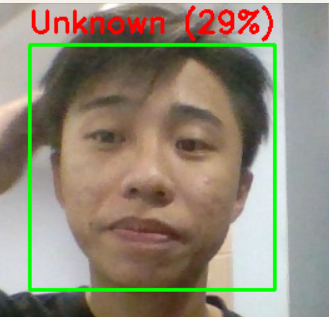
\includegraphics[width=0.2\textwidth]{nguoila.png}
    \caption{Kết quả nhận diện khuôn mặt từ File 03 bằng mô hình SVM}
    \label{fig:svm-test}
\end{figure}

\subsection*{Ghi nhận Check-in/Check-out thực tế}

Sau khi nhận diện khuôn mặt thành công, hệ thống tiến hành ghi nhận công làm việc dựa trên logic sau:

\begin{enumerate}
    \item \textbf{Truy vấn bảng Attendance} xem nhân viên đã có bản ghi trong ngày hay chưa.
    \item Nếu \textbf{chưa có} bản ghi:
    \begin{itemize}
        \item Hệ thống tạo mới một bản ghi \textbf{Check-in},Nhân viên thực hiện trong 15s và sau 30s có thể checkout.
        \item Lưu thời gian vào cột \texttt{TimeIn}.
    \end{itemize}
    \item Nếu \textbf{đã có} bản ghi:
    \begin{itemize}
        \item Hệ thống cập nhật thời gian vào cột \texttt{TimeOut}.
    \end{itemize}
    \item Độ tin cậy < 0.55 → hệ thống không ghi điểm danh và gán nhãn \textit{Unknown}. Ngưỡng 0.55 được chọn vì cho khả năng phát hiện người lạ tốt qua thực nghiệm, đồng thời vẫn nhận diện chính xác nhân viên nhằm hạn chế nguy cơ kẻ lạ đột nhập.

\end{enumerate}

Hệ thống đảm bảo:
\begin{itemize}
    \item Không ghi trùng Check-in hoặc Check-out.  
    \item Thông tin được lưu đầy đủ: ID, thông tin nhân viên, thời gian, độ tin cậy.  
\end{itemize}

\subsection*{Nhận xét}
\begin{itemize}
    \item Hệ thống nhận diện chính xác 100\% các khuôn mặt thuộc nhân viên có trong cơ sở dữ liệu.
    \item Các trường hợp người lạ được loại bỏ đúng nhờ ngưỡng tin cậy 0.55.
    \item Xác suất dự đoán trung bình cao, ổn định ngay cả khi ảnh File 03 có độ sáng và góc nhìn khác ảnh huấn luyện.
    \item Thời gian xử lý trung bình khoảng \textbf{0.07 giây/ảnh}, đáp ứng yêu cầu real-time.
    \item Bounding box ổn định, độ nhiễu thấp và không phát sinh nhầm lẫn chéo giữa các nhân viên.
    \item Chức năng \textbf{Check-in/Check-out} hoạt động chính xác, tự động hoá hoàn toàn quy trình điểm danh.
\end{itemize}

\section{Kết luận tạm thời}
Từ các kết quả thực nghiệm trên:
\begin{itemize}
    \item \textbf{SVM (RBF Kernel)} là mô hình tối ưu cho hệ thống nhận diện khuôn mặt trong bài toán điểm danh.
    \item Các phương pháp không giám sát như Cosine và L2 phù hợp khi dữ liệu ít nhưng không thay thế được SVM trong hệ thống thực tế.
    \item Toàn bộ pipeline từ nhận diện đến ghi nhận công làm việc vận hành ổn định, chính xác và đủ nhanh cho triển khai thật.
\end{itemize}

% Chương 4: Kết luận
\chapter{Kết luận}

\section{Kết luận \& Hướng phát triển}

Hệ thống đã xây dựng thành công một pipeline nhận diện khuôn mặt phục vụ điểm danh tự động, 
Dựa trên kết quả đạt được, hệ thống hoàn toàn đáp ứng yêu cầu triển khai thực tế trong môi trường doanh nghiệp với độ chính xác và tốc độ xử lý tốt.

\subsection*{Hướng phát triển}
\begin{itemize}
    \item Tích hợp cơ chế \textbf{liveness detection} nhằm chống giả mạo bằng ảnh, video hoặc thiết bị hiển thị.
    \item Nâng cấp mô hình trích xuất đặc trưng sang các kiến trúc mạnh hơn như \textbf{FaceNet}, \textbf{ArcFace} hoặc backbone hiện đại khi mở rộng dữ liệu.
    \item Phát triển ứng dụng \textbf{mobile} hoặc xây dựng \textbf{REST API} để triển khai đa nền tảng.
    \item Mở rộng hệ thống cho \textbf{tập dữ liệu lớn}, hỗ trợ nhiều nhân viên, nhiều camera và nhiều khu vực điểm danh.
    \item Tối ưu thời gian xử lý bằng các công nghệ như \textbf{TensorRT} hoặc \textbf{ONNX Runtime} để đảm bảo real-time trong môi trường tải cao.
\end{itemize}


\begin{thebibliography}{9}

\bibitem{opencv} OpenCV Development Team, \emph{OpenCV: Open Source Computer Vision Library}, \url{https://opencv.org/}, truy cập 2025.

\bibitem{viola-jones} P. Viola and M. Jones, ``Rapid Object Detection using a Boosted Cascade of Simple Features,'' \emph{Proceedings of CVPR}, 2001, trang 511--518.

\bibitem{mobilenetv2} M. Sandler, A. Howard, M. Zhu, A. Zhmoginov, L.-C. Chen, ``MobileNetV2: Inverted Residuals and Linear Bottlenecks,'' \emph{Proceedings of CVPR}, 2018, trang 4510--4520.

\bibitem{sklearn} F. Pedregosa et al., ``Scikit-learn: Machine Learning in Python,'' \emph{Journal of Machine Learning Research}, vol. 12, pp. 2825–2830, 2011.

\bibitem{keras} F. Chollet, \emph{Keras}, \url{https://keras.io/}, truy cập 2025.

\bibitem{tensorflow} M. Abadi et al., ``TensorFlow: Large-Scale Machine Learning on Heterogeneous Systems,'' 2015, \url{https://www.tensorflow.org/}.

\bibitem{streamlit} Streamlit Development Team, \emph{Streamlit Documentation}, \url{https://docs.streamlit.io/}, truy cập 2025.

\end{thebibliography}


% Phụ lục (Tùy chọn)
\appendix
\chapter{Phụ lục}
% [Thêm kết quả bổ sung, đoạn mã hoặc hướng dẫn sử dụng tại đây.]

\end{document}
